Uma célula fotovoltaica é basicamente uma junção P–N exposta à luz, o que possibilita conversão da energia
luminosa em energia elétrica.

Como essa junção funciona, essencialmente, como um diodo de silício, a tensão gerada é muito baixa, e a relação entre
tensão e corrente apresenta um comportamento fortemente não linear.


A \figr{fig:cell} ilustra um modelo equivalente da célula na forma de um circuito eletrônico.
Nesse modelo, a fonte de corrente e o diodo representam a dependência da célula em relação à irradiância e à temperatura.
\begin{figure}[htbp]
    \centering
    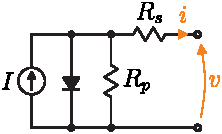
\includegraphics[scale=0.9]{figs/cell}
    \caption{Modelo de uma célula fotovoltaica.}
    \label{fig:cell}
\end{figure}

O circuito da \figr{fig:cell} pode ser equacionado por \eq{eq:cell}, onde $I$, $S$ e $T$ dependem das
características construtivas da célula além da irradiância e temperatura.
Ou seja, a rigor, esses parâmetros variam com as condições de operação às quais a célula é submetida.
Neste exercício, para fins de simplicidade, considere-os constantes.
\begin{equation}
    \textcolor{civ}{i} = I - S \left(
    e^{\dfrac{\textcolor{civ}{v} -\textcolor{civ}{i}  R_s}{T}} - 1
    \right) - \dfrac{\textcolor{civ}{v} -\textcolor{civ}{i}  R_s}{R_p}
    \label{eq:cell}
\end{equation}

A resolução da \eq{eq:cell} permite calcular a corrente, a tensão e, por consequência, a potência gerada para uma
determinada condição de irradiância e temperatura.
A principal dificuldade nessa resolução está na interdependência do termo exponencial com a tensão e a corrente da
célula, o que torna a equação transcendental, impedindo o isolamento direto de $i$.
Dessa forma, a solução só pode ser obtida por meio de métodos numéricos, utilizando aproximações sucessivas.

Diversos métodos numéricos podem ser utilizados para resolver a \eq{eq:cell}.
Em particular, o método de Newton permite obter uma solução aproximada por meio de iterações sucessivas, atualizando
a estimativa a cada passo.
Se o método convergir, essa nova estimativa tende a se aproximar progressivamente da solução exata.
Aplicando o método de Newton à \eq{eq:cell}, obtém-se:
\begin{equation}
    i_{\0} = i_{\1} - \delta{\1}
    \label{eq:newton}
\end{equation}
sendo
\begin{equation}
    \delta\0 =  \myfrac[1.1em]{I - S  \cdot \exp \left( \dfrac{v- R_s \cdot i\0}{T} - 1 \right) - \dfrac{v- R_s \cdot i\0}{R_p} - i\0}
    {-1 - \dfrac{S\cdot R_s}{T} \cdot \exp \left( \dfrac{v- R_s \cdot i\0}{T} \right) - \dfrac{R_s}{R_p} }
    \label{eq:newton2}
\end{equation}


A estimativa da corrente, dada por \eq{eq:newton}, deve ser atualizada iterativamente para $n = 1, 2, \ldots$, até
que o valor absoluto de $\delta_n$ seja inferior à tolerância estabelecida.
Em outras palavras, as equações \eq{eq:newton} e \eq{eq:newton2} devem ser aplicadas sucessivamente
enquanto $\left| \delta_n \right| > \epsilon$.

Como se trata de um método iterativo, cada nova estimativa da corrente depende da anterior.
Assim, o cálculo de $i_1$ requer o conhecimento prévio de $i_0$.
Para iniciar o algoritmo, assume-se $i_0 = 0$.

\subsection*{Etapa 1}

Escreva uma função \inlcode{i_cell(v: float) -> float} que calcule e retorne a corrente da célula para uma dada
tensão passada como argumento.

Utilize as seguintes constantes:
\begin{table}[!hp] \centering
\begin{tabular}{c c c}
símbolo & valor & U.M. \\ \hline
$R_s$ & 0.002 & \Omega \\
$R_p$ & 10.0 & \Omega \\
$I$ & 8.0 & A \\
$S$ & 0.02 & A \\
$T$ & 0.085 & V \\
$\epsilon$ & 0.001 & A \\ \hline
\end{tabular}
\end{table}

Um teste inicial da função gerada pode ser realizado com:
\begin{minted}{custompython}
def i_cell(v: float) -> float:
    # seu código aqui

print(f"{i_cell(0.4) = }")
print(f"{i_cell(0.5) = }")
\end{minted}
\begin{minted}{text}
i_cell(0.4) = 7.275763496758507
i_cell(0.5) = 5.64008091541083
\end{minted}

\subsection*{Etapa 2}
Uma vez realizada essa validação inicial, escreva um script que traçe uma curva da corrente em
função da tensão nos terminais da célula tensão.
O script deve gerar uma figura semelhante a da \figr{fig:pv}.
\begin{figure}[htbp]
    \centering
    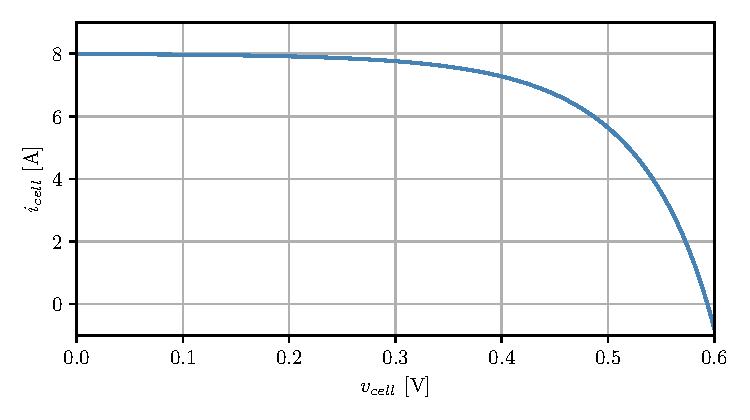
\includegraphics[scale=1.0]{figs/pvcell}
    \caption{Resultado gráfico esperado do script para teste de \inlcode{i_cell}.}
    \label{fig:pv}
\end{figure}


\subsection*{Etapa 3}
Utilize algum método do pacote \inlcode{scipy.optimize} obter o ponto de máxima potência, e represente-o no gráfico
de potência por tensão da célula    .
O script deve gerar uma figura semelhante a da \figr{fig:pvotp}.
\begin{figure}[htbp]
    \centering
    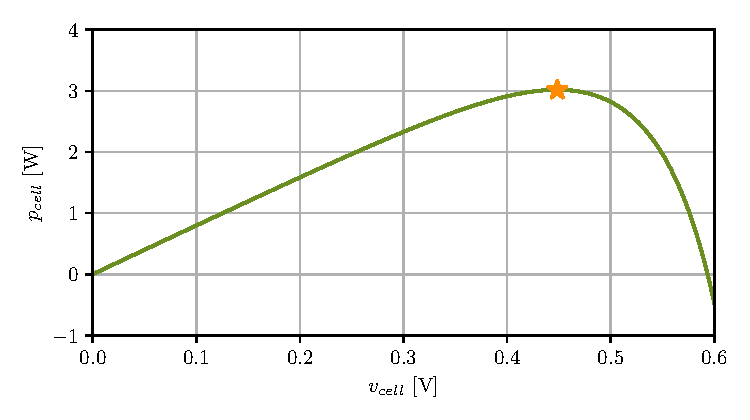
\includegraphics[scale=1.0]{figs/pvcellotp}
    \caption{Resultado gráfico esperado do script de MPP.}
    \label{fig:pvotp}
\end{figure}